% SPDX-FileCopyrightText: 2026 Will Cook
% SPDX-License-Identifier: CC-BY-4.0
\documentclass[11pt]{article}
\usepackage[T1]{fontenc}
\usepackage[utf8]{inputenc}
\usepackage[a4paper,margin=1in]{geometry}
\usepackage{amsmath,amssymb,booktabs,array,graphicx}
\usepackage[dvipsnames]{xcolor}
\usepackage{tikz}
\usetikzlibrary{arrows.meta,positioning,calc}
\usepackage[colorlinks=true,linkcolor=black,urlcolor=RoyalBlue,citecolor=black]{hyperref}
\hypersetup{
  pdftitle={Claim-Faithful Publication of a Formalised Mathematics Corpus},
  pdfauthor={Will Cook},
  pdfsubject={A case study in release-time claim-strength governance: status registries, verified source anchors, budgeted projections, and a self-testing release gate},
}
\newcommand{\commit}{a16aa24af5236b6508a34b8a4c4b41fdcf620a98}
\newcommand{\repobase}{https://github.com/wcook04/plectis-lean-erdos249-257/blob/\commit}
\newcommand{\file}[2]{\href{\repobase/#1}{#2}}
\newcommand{\state}{\mathcal{A}}
\newcommand{\mutset}{\mathcal{M}}
\emergencystretch=2em
\title{Claim-Faithful Publication of a Formalised\\ Mathematics Corpus\\
{\large A case study in release-time claim-strength governance}}
\author{Will Cook}
\date{July 2026}

\begin{document}
\sloppy
\maketitle

\begin{abstract}
A proof assistant verifies exactly the propositions its kernel elaborates, at
exactly the stated generality; publication begins where that guarantee stops.
Everything a project says about a formal development --- papers, a README,
orientation files, machine-readable packets --- restates the mathematics
outside the kernel, and the characteristic restatement failure is silent
strengthening: an implication reads as an equivalence, finite evidence reads
as an unbounded theorem, an open problem quietly leaves the page.  We present
a case study in release-time claim-strength governance for a Lean corpus of
$12{,}496$ declarations around two open Erd\H{o}s problems.  A pinned
formal-source checkpoint; a typed claim registry in which formal claims must
carry kernel-checked declarations at pinned coordinates and open or cited-only
claims must not carry any; authored papers whose prose holds verified source
anchors inside ordinary mathematical phrases; and bounded generated reader
surfaces are checked together by one release gate --- $5{,}207$ checks at the
studied checkpoint --- which also runs its own detectors against planted
corruptions, so a detector that stops detecting is itself a release failure.
In a ten-mutation study at that checkpoint the gate rejected nine deliberate
corruptions.  The tenth, a one-clause strengthening of a finite-evidence
boundary that no declared invariant had named, passed every check; its repair
became a new anchor with a permanently derived rejection fixture.  The
contribution is neither a semantic checker for arbitrary prose nor a
mathematical theorem: it is an implemented, evaluated, and deliberately
bounded contract for keeping the logical status and open boundaries of one
formal corpus stable across the surfaces through which people and machines
actually read it.  We conjecture that the failure classes recur wherever
public prose restates machine-checked content; transfer beyond this corpus is
untested.
\end{abstract}

\section{Introduction}\label{sec:sys-intro}

The Lean kernel accepts a proof term for a stated proposition.  That
acceptance is narrow and exact: it covers the elaborated statement, under the
stated hypotheses, at the stated generality, and nothing else.  A formal
development of useful size, however, is not read through its kernel.  It is
read through publication surfaces: an expository paper, a README, a scope
statement, orientation documents, navigation indices, and increasingly through
bounded machine-readable packets consumed by software agents.  Each surface
restates the mathematics in a form the kernel never sees, and each restatement
can strengthen a claim without anyone deciding to strengthen it.

The corpus studied here formalises results around Erd\H{o}s problems 249 and
257, two open irrationality questions.  Both problems remain open, and the
corpus says so; its value depends on saying so in every restatement.  This
creates an unusually sharp version of a general problem.  A library of settled
mathematics that misdescribes a theorem's strength embarrasses its authors.  A
corpus organised around open problems that misdescribes a conditional
reduction as a proof, or lets a verified finite range read as an unbounded
quantifier, damages the one thing it exists to establish: an exact public
boundary between what is proved and what is not.

The response studied here is to make claim strength a machine object and to
check it at release time.  A registry types every public claim with one of
seven logical statuses; the authored papers carry their formal anchors inside
ordinary mathematical phrases; every navigation surface is generated,
digest-chained, and byte-budgeted; and one command validates the whole
arrangement, including its own detectors.  The sharpest evidence in this paper
--- for the value of that arrangement and for its exact limit --- is a single
sentence.  A mutation study planted ten corruptions, one at a time, at a
checkpoint where all $5{,}207$ checks pass.  Nine were rejected.  The tenth
--- mutation M8 in the study's numbering ---
weakened one boundary clause in the README, replacing ``does not supply the
unbounded quantifier'' by ``completes the unbounded quantifier'', and every
check passed, because no declared invariant had named that clause.  The repair
used the architecture's own idiom: the clause became a semantic anchor group,
the comprehension suite derived a rejection mutant from it automatically, and
the same corruption now fails the gate
(Figure~\ref{fig:escape}).  Declared boundaries are executable; undeclared
semantics stay outside the contract.  This paper is organised around that
line.

The claims of this paper are about the invariants, not the implementation
effort.  Its components are ordinary --- a JSON registry, some authored
\TeX{}, generated Markdown, and roughly $7{,}800$ lines of dependency-free
Python --- and that ordinariness is part of the point:

\begin{enumerate}
\item \emph{A recorded authority order} (Section~\ref{sec:authority}).  Proof
  authority, claim-status authority, methodological authority, authored
  exposition, and generated navigation are distinct layers, machine-recorded
  in that order; a surface may compress or omit what it inherits from the
  layers above and must not strengthen it.  Each evidence class must record
  what it does \emph{not} decide.
\item \emph{Claim status as a typed machine object}
  (Section~\ref{sec:registry}).  Every public claim carries one of seven
  statuses with structural rules (an open or cited-only claim must not carry
  proof declarations; every other claim must), every remaining open
  proposition is a typed record, and the registry also carries explicit
  \emph{non-claims}.  All $96$ claims are partitioned exactly once into $20$
  contribution families, and the partition is checked.
\item \emph{Anchored exposition} (Section~\ref{sec:anchors}).  Paper prose
  links each stated result to a pinned commit, file, line, and declaration;
  the visible text is an ordinary mathematical phrase, the coordinates
  underneath are validated to within a three-line window, and the rendered
  mathematics is forbidden from printing raw paths, hashes, or Lean
  identifiers.  Every remaining open proposition must resolve to exactly one
  authored problem statement, so an open problem cannot be dropped from the
  exposition without the gate failing.
\item \emph{Budgeted projections} (Section~\ref{sec:projections}).  Generated
  reader surfaces are rebuilt from the registry by named owners, tied together
  by content digests, and held under explicit byte budgets, so first contact
  stays readable as the corpus grows.
\item \emph{A self-testing release gate} (Sections~\ref{sec:model},
  \ref{sec:gate}, and~\ref{sec:eval}).  One command runs $5{,}207$ checks in
  $144.5$ seconds at the studied checkpoint and fails on untrusted proof
  code, status drift, boundary loss, coordinate rot, stale projections, or
  budget overflow.  Sixty-nine negative fixtures run inside the gate against
  the gate's own checkers.  In the mutation study of
  Section~\ref{sec:eval}, nine of ten deliberate corruptions were detected
  and the escape was converted into a new anchor and fixture; during ordinary
  development the same machinery caught three real defects, including an edit
  that deleted a load-bearing negative sentence.
\end{enumerate}

Two boundaries on these claims should be stated at once and are developed in
Sections~\ref{sec:model} and~\ref{sec:limits}.  First, this is a case study
of one corpus with one maintainer; no controlled comparison against
conventional practice is attempted.  Second, the gate checks the declared
invariants and nothing else: it establishes presence, agreement, and
freshness for enumerated sentences, fields, coordinates, and digests, and it
does not judge the mathematical adequacy of unanchored prose.  The
architecture makes a specific class of publication defects mechanically
detectable at commodity cost; it does not make exposition true.

On provenance: the development and its tooling were built by a single
maintainer working with AI assistants; the Lean kernel, not any assistant, is
the proof authority, and the release machinery described here exists partly
\emph{because} assistant-generated edits are a real source of drift.  Two of
the three development defects recorded in Section~\ref{sec:receipts} were
introduced by tooling-assisted editing passes and caught by the gate.

\section{The published corpus}\label{sec:corpus}

The artifact is a public Lean~4 package~\cite{lean} building against
Mathlib~\cite{mathlib}, together with its publication surfaces.  Two commits
identify the studied state.  The registry pins a \emph{formal-source
checkpoint} (commit \texttt{a16aa24}), the exact Lean tree that owns every
claimed declaration; paper links resolve into that immutable tree.  The
\emph{evaluation checkpoint} (commit \texttt{0e5aaf9}) is the later repository
state at which the study of Section~\ref{sec:eval} ran: its Lean surface is
identical to the formal-source checkpoint --- the gate enforces that identity
--- and all $5{,}207$ release checks pass there.  Counts in this paper are
stamped at the evaluation checkpoint and grow under development.

At that checkpoint the corpus comprises $633$ Lean modules and $12{,}496$
declarations; $11{,}471$ of the declarations are theorem-like, and $2{,}925$
of those are generated finite-certificate declarations.  The registry curates $96$ public claims in
$20$ contribution families, three typed remaining-open propositions, and six
non-claims.  The mathematical content --- exact certificate equivalences,
sharp denominator bounds, achievement-set geometry, and scoped countermodels
for the two Erd\H{o}s problems --- is the subject of the gateway
exposition~\cite{mainpaper} and the transport--curvature
companion~\cite{companion}; this paper does not restate it and claims no
mathematical results.

The division of labour among the three papers is deliberate.  The gateway owns
the mathematics; the companion owns one specialist programme; this paper owns
the question of how a corpus of that size is published without its
restatements outrunning its proofs.  The mathematics serves here only as the
live instance on which the machinery is exercised.  We conjecture that the
failure classes below recur wherever public surfaces restate kernel-checked
content; this corpus supplies evidence that they occur, not that the response
transfers.

\section{The failure model}\label{sec:failure}

The architecture is organised against five concrete ways a truthful corpus
drifts into an untruthful publication.  All five were either observed in this
project's development or are one careless edit away; none requires bad faith.

\emph{Status inflation.}  A conditional reduction is summarised as a result;
a one-way implication is remembered as the equivalence it almost is; a
verified finite range is described with the unbounded quantifier it supports
only conditionally.  The opposite defect is quieter but also real:
understatement, as when a proved equivalence is cautiously reported as a
sufficient condition.  Both directions misstate the mathematics; an exact
status vocabulary must resist both.

\emph{Boundary erosion.}  The sentences that carry negative information ---
``this does not solve the problem'', ``this bound does not supply the
unbounded quantifier'' --- are precisely the ones a well-meaning copy edit
deletes, because they read as redundant hedging to anyone who has not
internalised why they are load-bearing.

\emph{Coordinate rot.}  Links from prose to source are correct on the day
they are written.  Source moves; line numbers shift; a renamed module orphans
a hundred references.  A reader who follows a stale anchor to the wrong
declaration has been misinformed as surely as by a wrong sentence.

\emph{Projection fossilisation.}  Generated summaries, indices, and counts
are rebuilt when someone remembers to rebuild them.  A hand edit to a
generated file, or a forgotten rebuild after an upstream change, leaves two
public surfaces asserting different facts.

\emph{Attention overflow.}  First-contact surfaces grow monotonically under
ordinary maintenance, until the document that was supposed to orient a reader
in one minute no longer can.  Unbounded growth is a truthfulness problem, not
only a style problem: a boundary sentence that has scrolled out of the part
people read might as well have been deleted.

\begin{figure}[t]
\centering
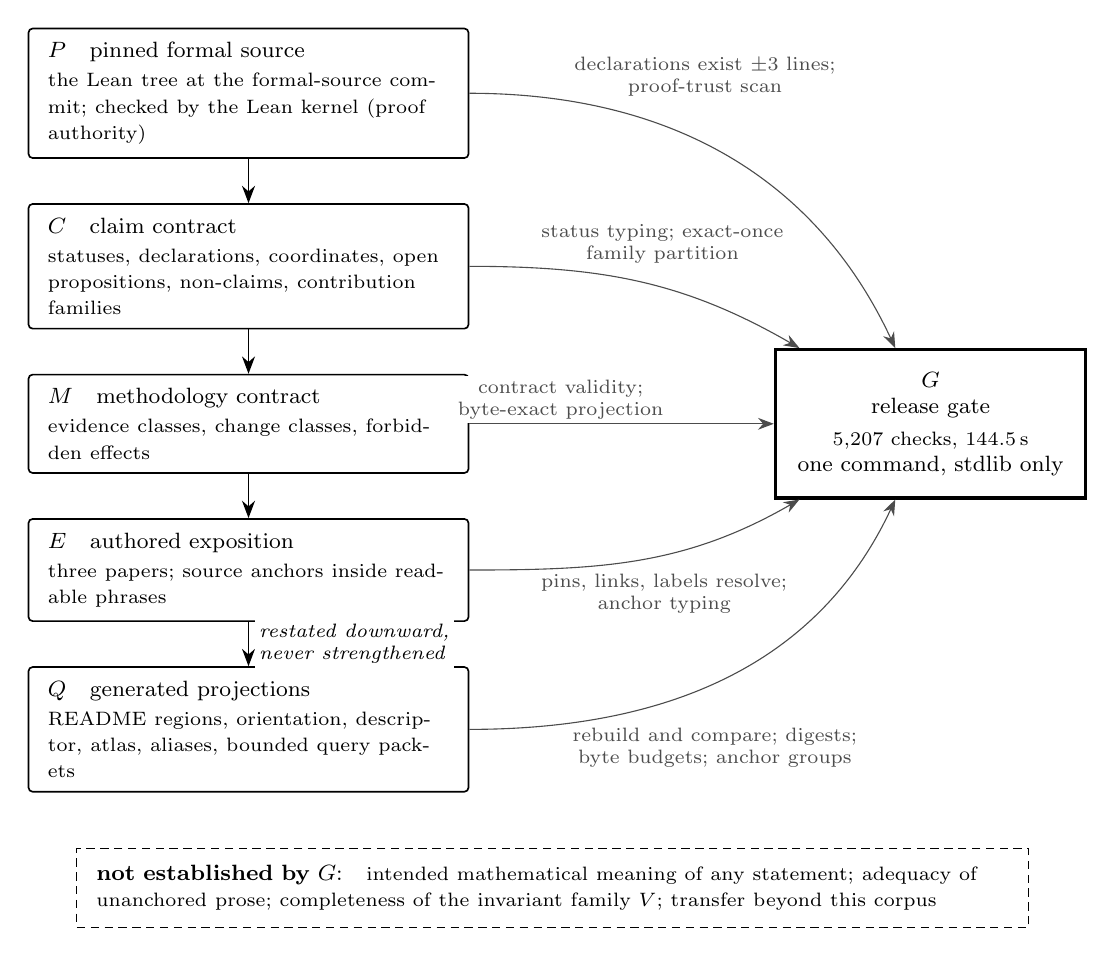
\begin{tikzpicture}[
  font=\footnotesize,
  owner/.style={draw, semithick, rounded corners=1.5pt, align=left,
    inner xsep=7pt, inner ysep=5pt, text width=14.5em},
  gatebox/.style={draw, very thick, align=center, inner sep=8pt},
  residue/.style={draw, densely dashed, align=left,
    inner xsep=7pt, inner ysep=6pt, text width=15em},
  restate/.style={-{Stealth[length=2.2mm]}, semithick},
  checkarc/.style={-{Stealth[length=2mm]}, gray!60!black},
  clab/.style={font=\scriptsize, fill=white, inner sep=1.5pt, align=center}
]
\node[owner] (P) {$P$\quad pinned formal source\\[1pt]
  {\scriptsize the Lean tree at the formal-source commit;
   checked by the Lean kernel (proof authority)}};
\node[owner, below=1.6em of P] (C) {$C$\quad claim contract\\[1pt]
  {\scriptsize statuses, declarations, coordinates, open propositions,
   non-claims, contribution families}};
\node[owner, below=1.6em of C] (M) {$M$\quad methodology contract\\[1pt]
  {\scriptsize evidence classes, change classes, forbidden effects}};
\node[owner, below=1.6em of M] (E) {$E$\quad authored exposition\\[1pt]
  {\scriptsize three papers; source anchors inside readable phrases}};
\node[owner, below=1.6em of E] (Q) {$Q$\quad generated projections\\[1pt]
  {\scriptsize README regions, orientation, descriptor, atlas, aliases,
   bounded query packets}};

\draw[restate] (P.south) -- (C.north);
\draw[restate] (C.south) -- (M.north);
\draw[restate] (M.south) -- (E.north);
\draw[restate] (E.south) -- (Q.north)
  node[clab, midway, right=2pt, align=left]
  {\itshape restated downward,\\ \itshape never strengthened};

\node[gatebox, right=11em of M] (G) {$G$\\ release gate\\[2pt]
  \scriptsize $5{,}207$ checks, $144.5$\,s\\ one command, stdlib only};

\draw[checkarc] (P.east) to[out=0, in=115]
  node[clab, pos=0.18, anchor=south west]
  {declarations exist $\pm3$ lines;\\ proof-trust scan}
  (G.115);
\draw[checkarc] (C.east) to[out=0, in=150]
  node[clab, pos=0.18, anchor=south west]
  {status typing; exact-once\\ family partition}
  (G.150);
\draw[checkarc] (M.east) --
  node[clab, pos=0.30, anchor=south]
  {contract validity;\\ byte-exact projection}
  (G.180);
\draw[checkarc] (E.east) to[out=0, in=210]
  node[clab, pos=0.18, anchor=north west]
  {pins, links, labels resolve;\\ anchor typing}
  (G.210);
\draw[checkarc] (Q.east) to[out=0, in=245]
  node[clab, pos=0.18, anchor=north west]
  {rebuild and compare; digests;\\ byte budgets; anchor groups}
  (G.245);

\node[residue, anchor=north, text width=33em]
  at ($(Q.south)+(11em,-2.0em)$) (R)
  {\textbf{not established by $G$}:\quad
  {\scriptsize intended mathematical meaning of any statement; adequacy of
   unanchored prose; completeness of the invariant family $V$; transfer
   beyond this corpus}};
\end{tikzpicture}
\caption{The publication state $\state=(P,C,M,E,Q)$ and the release predicate
$G$ at the evaluation checkpoint.  Layers on the left are believed in
top-to-bottom order; each lower surface restates the mathematics and must not
strengthen what it inherits.  Each arrow into $G$ names the contract the gate
checks for that layer.  The dashed box lists what a passing gate does
\emph{not} establish; Section~\ref{sec:eval} exhibits one sentence that
escaped through exactly that residue.}
\label{fig:contract}
\end{figure}

\section{Authority order}\label{sec:authority}

The registry records, as data, the order in which surfaces may be believed
(Figure~\ref{fig:contract}): first Lean source checked by the pinned kernel;
second the claim registry (\texttt{docs/claims.json}) for release identity,
status taxonomy, remaining open propositions, coordinates, and navigation
relationships; third the methodology contract
(\texttt{docs/methodology.json}); fourth the authored exposition; and last the
README, scope, and navigation documents as reader projections.  Two
disciplines make this order load-bearing rather than decorative.

First, \emph{no strengthening downstream}: a surface may compress or omit
what it inherits, and may never assert a stronger logical status than the
layer above it records.  The gate implements this obligation directionally
and pointwise --- every downstream surface is checked against the registry,
and the registry against the pinned Lean tree, for the sentences, fields, and
coordinates the invariants enumerate --- so within the enumeration, an
overstatement must appear upstream, in the one place designed to be reviewed
line by line, or be caught.  Outside the enumeration nothing is promised;
Section~\ref{sec:eval} measures exactly one such miss.

Second, \emph{explicit non-decision}.  The methodology contract types its
evidence classes (kernel check, repository check, human mathematical review),
and each class must state both what it decides and what it does not decide;
the contract validator rejects an evidence class missing either field.  The
same posture appears at the top of the order as a method axiom: kernel
acceptance establishes the elaborated proposition, not that the proposition
expresses the intended mathematics.  Making every authority state its own
boundary is the single design decision from which most of the machinery below
follows.

The registry also records six explicit \emph{non-claims}, three of which are
provenance boundaries: the public corpus is a self-contained projection of a
larger private research workflow, and the registry states as checkable data
that no public claim rests on hidden proof bodies, private repositories, or
any authority other than the pinned public sources.  The comprehension suite
of Section~\ref{sec:gate} fails if these non-claims, or the plain-language
sentences that carry them, disappear from the entry surfaces.

\section{Claim status as a typed object}\label{sec:registry}

Each of the $96$ public claims carries one status from a closed taxonomy of
seven, and the taxonomy itself records a meaning sentence per status:
\emph{proved here}, \emph{formalised here}, \emph{unconditional progress}
(``genuine theorem that does not settle the open problem''), \emph{conditional
reduction} (``exact implication whose remaining hypothesis is open''),
\emph{verified finite instance} (``kernel-checked computation at a bounded
range''), \emph{cited only}, and \emph{open}.  The taxonomy is deliberately
finer than proved/unproved, because the corpus's characteristic outputs ---
exact equivalences whose producers remain open, kernel-checked certificate
ranges, denominator exclusions that bound without deciding --- are exactly the
results that coarse vocabularies inflate.

Statuses are structurally typed, not just enumerated.  A claim whose status is
\emph{cited only} or \emph{open} must not carry proof declarations; every
other claim must carry at least one, and each declaration names a module and
line at which the declaration is verified to exist, against the pinned
formal-source commit rather than the working tree.  Remaining open
propositions are first-class records, and any claim asserting progress toward
one must name its effect from a closed vocabulary --- \emph{proves},
\emph{narrows}, \emph{decomposes}, \emph{re-expresses}, or \emph{constrains}
--- so that ``progress'' cannot be claimed without saying what changed.

The methodology contract extends the same typing to \emph{changes}.  Eleven
change classes (proof body changed, assumptions changed, finite certificate
range changed, claim status changed, and so on) each carry minimum evidence
requirements and forbidden effects.  Two examples fix the flavour: a change of
class \emph{finite certificate range changed} is forbidden from carrying the
effect \emph{infer unbounded result}, and any change class that alters
mathematical semantics is forbidden from downgrading human mathematical
review to an automatic trigger.  A rule in the contract must name the release
guard that implements it, and the rendered \texttt{METHODOLOGY.md} must match
its JSON source byte for byte.

Finally, the registry partitions all claims into $20$ contribution families,
each with a narrative owner, a status summary, a prior-art posture, and an
open obligation or consumer.  The gate enforces that the families cover every
claim exactly once.  The partition exists for editorial honesty: a claim that
belongs to no family has no owner responsible for stating its boundary, and a
claim in two families gets described twice, which is how wording divergence
starts.

\section{Anchored exposition}\label{sec:anchors}

The authored mathematics papers link prose to source through four macros
whose visible output is ordinary text and whose arguments carry the exact
coordinates underneath.  In the gateway paper, the two default macros turn
the declaration name into a spaced, lower-case label; the third prints a
chosen semantic label --- so a theorem is cited as, say, the
\emph{tail-difference equivalence} --- and the fourth prints ``Lean source''.
The companion retains the quieter ``Lean proof'' fallback.  The papers pin
the full formal-source commit; links resolve into that immutable tree, never
into a floating branch.  The release gate re-validates every link: the file
must exist at the pinned commit and the named declaration must appear within
three lines of the stated coordinate.

Anchoring is bidirectional.  Downward, each claim in the registry may name
the paper label that presents it, and the gate fails if the label does not
exist in the authored \TeX{}.  Upward, an inventory derives every anchor in
the papers --- labelled sections and formal environments --- and types each
one as a registered claim anchor, a remaining-open-proposition anchor, an
authored formal anchor without a registered claim, or a navigation anchor.
Two consequences of this typing carry most of the value.  Every remaining
open proposition must resolve to exactly one authored problem environment
across the paper suite: an open problem cannot be dropped from the exposition,
or duplicated into two competing statements, without the gate failing.  And
the anchor classes let the gate reject a problem statement that has quietly
stopped being typed as open.

A rendering contract keeps the implementation layer out of the printed
mathematics, in two modes.  Inside the release gate, a source-mode check
requires each link macro to print readable words and forbids the visible
\TeX{} of the mathematics papers from containing implementation paths,
forty-character hashes, or raw identifier macros.  At build time, a full-mode
check extracts the rendered PDF text and rejects internal file names, module
names, and source sigils, and enforces a \emph{first-minute contract}: named
boundary phrases --- among them ``neither problem is settled'' and ``an
unbounded certificate supply'' --- must appear on named early pages of each
mathematics paper, so the load-bearing negative sentences provably survive
into what a first-time reader actually sees.  The contract is scoped to the
two mathematics papers by role: the present paper's subject is the
implementation, so file and script names appear here deliberately, and this
paper sits outside that checker rather than weakening it.

\section{Budgeted projections}\label{sec:projections}

Everything a reader or an agent meets before the papers is generated: the
orientation documents, the corpus descriptor, the declaration atlas, the
README's scale and anchor regions, and the bounded query interface.  Three
rules govern this layer.

\emph{Builders own generated regions.}  Generated files and regions are
marked, rebuilt by named scripts, and compared byte-for-byte in the gate; a
hand edit to a generated surface is a release failure by construction.
Content digests tie the layers together --- the descriptor records SHA-256
digests of the mathematics papers' sources, their rendered PDFs, and the
alias crosswalk --- so a digest-recorded artifact cannot silently represent a
newer source.

\emph{First contact is budgeted.}  The README's first-contact region must fit
in $12{,}000$ bytes, the scope statement in $4{,}000$, the human orientation
document in $16{,}000$, the machine orientation capsule in $32{,}000$, the
corpus descriptor in $64{,}000$, and any entry route's total first-contact
bundle in $48{,}000$; the bounded query tool caps each packet at $16{,}384$
bytes and a summary at $32{,}000$.  Budgets are enforced in the gate, so
surface growth becomes a visible editorial decision --- compress or re-route
--- rather than silent accretion.  Twice during development a budget failed
and was met by removing duplication rather than by raising the number; both
incidents are recorded in Section~\ref{sec:receipts}.

\emph{Entry routes must be bounded.}  Machine entry points are typed routes
with intents, bounded reads, and query steps; a route is forbidden from
sending first contact to an exhaustive owner such as the full registry or the
declaration atlas.  Programme-level routes must additionally state an
explicit negative claim ceiling --- the checker literally requires wording
such as ``remain open'' or ``does not'' --- so that even the navigation layer
carries the open boundary.

\section{A minimal model of the contract}\label{sec:model}

The arrangement of Sections~\ref{sec:authority}--\ref{sec:projections} can be
stated in a few lines of notation; we introduce only what removes ambiguity.
Write
\[
\state \;=\; (P,\, C,\, M,\, E,\, Q)
\]
for the publication state: $P$ the pinned formal source, $C$ the claim
contract, $M$ the methodology contract, $E$ the authored exposition, and $Q$
the generated projections.  Let $V=\{v_1,\dots,v_k\}$ be the \emph{declared
invariant family}: each $v_j$ is an executable predicate over $\state$ ---
a declaration exists within three lines of its coordinate, a status carries
no forbidden declarations, a generated file equals its rebuild, a budget
holds, a named sentence is present.  The release predicate is the
conjunction
\[
G(\state) \;=\; \bigwedge_{j=1}^{k} v_j(\state).
\]

Three readings of $G(\state)=1$, stated exactly.  It means every declared
invariant holds.  It does not mean any sentence of $E$ or $Q$ is
mathematically adequate: the $v_j$ quantify over enumerated sentences,
fields, coordinates, and digests, and a sentence outside the enumeration is
outside the guarantee.  It does not move proof authority, which belongs to
$P$ under the kernel and is only \emph{inherited} by $C$, $E$, and $Q$.  And
it does not discharge the human-review obligation recorded in $M$: the
methodology contract forbids every semantic change class from downgrading
human mathematical review, so $G$ supplements that review and cannot replace
it.

The order of Section~\ref{sec:authority} is a non-strengthening obligation on
restatements: a downstream surface may omit or weaken what it inherits and
must not strengthen it.  $V$ implements the obligation pointwise, on the
restatements it enumerates; it is not a semantic theorem about $E$.

$V$ is itself under test inside $G$.  For a family $F$ of fixture mutants ---
pinned known-bad inputs for the proof-trust scanner, methodology mutations
that must fail contract validation, and one deletion mutant derived
automatically from every declared anchor group --- the gate requires each
$m\in F$ to be rejected, so a checker that silently stops detecting is itself
a release failure.

For a mutant set $\mutset$ applied to a state with $G(\state)=1$, write
\[
\mu_G(\mutset) \;=\;
\frac{\bigl|\{\,m\in\mutset : G(m(\state))=0\,\}\bigr|}{|\mutset|}
\]
for the observed detection ratio.  Section~\ref{sec:eval} reports
$\mu_G=9/10$ for the ten authored mutations at the evaluation checkpoint, and
separately reports the repair of the survivor.  The notation makes the
paper's central negative result visible: $G$ is exactly as broad as $V$.
Mutation M8 survived because no member of $V$ named the sentence it weakened,
and the repair extended $V$ rather than editing the mutated surface.

\section{The release gate}\label{sec:gate}

One command, \file{scripts/check_release.py}{the release checker}, is the
executable form of $G$: $5{,}207$ checks in $144.5$ seconds at the evaluation
checkpoint, implemented in dependency-free Python over the working tree and
the pinned Git history.  The gate begins with the cheapest high-severity
invariant: a proof-trust scan rejecting \texttt{sorry}, \texttt{admit},
project-defined axioms, and native evaluation in every Lean source, with
comment- and string-aware lexing so prose mentions do not mask executable
occurrences; if this scan fails, the gate aborts before any expensive
validation runs.  It then verifies, in order: registry well-formedness and
status typing; release identity across the build manifest, citation file, and
toolchain pin; the formal-source identity of the working Lean tree; the
existence and location of every claimed declaration at the pinned commit;
every paper source link; scope and README boundary sentences, including a
banned-phrase list and a leak check for internal machine identifiers;
licensing completeness; agent-entry routing; methodology contract validity
and projection identity; module-graph, atlas, coordinate, descriptor, and
alias freshness by rebuild-and-compare; the source mode of the rendered-paper
contract; descriptor and orientation invariants; and the bounded-query and
cold-clone comprehension suites.

The design decision that distinguishes the gate from a conventional test
suite is that it validates its own detectors.  At the evaluation checkpoint,
sixty-nine negative fixtures ran inside the gate: five pinned inputs hold the
proof-trust scanner to its lexical boundary (three executable
native-evaluation forms must be rejected; a comment and a string mention must
be ignored); nine methodology mutations --- a conditional reduction without a
remaining-open link, a finite result restated as open, a semantic change with
downgraded review, and six more --- must each fail contract validation; and
the cold-clone comprehension suite, after validating the real surfaces,
applies fifty-five semantic mutations --- one deletion mutant derived
automatically from every declared anchor group, plus authored corruptions of
the packet layer, from a claim ceiling rewritten to assert a solution to a
provenance boundary rewritten to admit private proof authority --- each of
which must be rejected.  A checker whose fixtures stop failing fails the
release.  This matters under maintenance: the easiest way to defeat a guard
is not to attack it but to weaken it while editing something nearby, and the
fixtures convert that regression into a visible failure.  The fixture census
grows with the checker: at the later tree current when this paper was written
(commit \texttt{67fc5e0}), the scanner pins twelve inputs and the suite
derives sixty-six cold-clone mutations.

\section{Evaluation}\label{sec:eval}

\subsection{Mutation study}\label{sec:mutation}

The study answers four questions in order: what the gate claims to check,
which planted corruptions exercise those claims, which corruption survived
and why, and what changed in the detector afterwards.

\emph{What the gate claims to check.}  The declared invariants of
Sections~\ref{sec:authority}--\ref{sec:gate} group into seven families:
proof trust; registry structure (status typing and the family partition);
source coordinates; paper anchoring; boundary language; projection freshness
(rebuild-and-compare with digest chaining); and byte budgets.

\emph{The protocol.}  An isolated worktree was pinned at the evaluation
checkpoint, where all $5{,}207$ checks pass in $144.5$ seconds.  Ten
mutations --- at least one per invariant family, written by the checker's
author --- were applied one at a time, running the full gate after each and
restoring the tree between runs.  Table~\ref{tab:matrix} reports, for each
mutation, the invariant family that detected it first, every additional
family that fired, and the wall-clock time of the run.

\begin{table}[t]
\centering\footnotesize
\setlength{\tabcolsep}{3.5pt}
\newcommand{\fst}{$\bullet$}
\newcommand{\alsofam}{$\circ$}
\begin{tabular}{@{}l l ccccccc r@{}}
\toprule
 & Mutation (applied alone)
 & \rotatebox{75}{proof trust}
 & \rotatebox{75}{registry}
 & \rotatebox{75}{coordinates}
 & \rotatebox{75}{anchoring}
 & \rotatebox{75}{boundary}
 & \rotatebox{75}{freshness}
 & \rotatebox{75}{budgets}
 & \rotatebox{75}{time (s)} \\
\midrule
M1  & status upgraded: \emph{conditional} $\to$ \emph{proved here}
    &  &  &  &  &  & \fst &  & $139.4$ \\
M2  & README open boundary deleted (``does not solve'')
    &  &  &  &  & \fst &  &  & $171.5$ \\
M3  & declaration coordinate drifted $+40$ lines
    &  &  & \fst &  &  & \alsofam &  & $239.1$ \\
M4  & paper source link retargeted $+50$ lines
    &  &  & \fst &  &  & \alsofam &  & $192.2$ \\
M5  & one claim placed in two families
    &  & \fst & \alsofam &  &  & \alsofam &  & $121.4$ \\
M6  & descriptor hand-edited (module count $+1$)
    &  &  &  &  &  & \fst &  & $184.8$ \\
M7  & \texttt{native\_decide} introduced into a proof
    & \fst &  &  &  &  &  &  & $4.7$ \\
M8  & boundary clause: ``does not supply'' $\to$ ``completes''
    & \multicolumn{7}{c}{\emph{escaped: all checks passed}}
    & $176.0$ \\
M9  & open-problem anchor title mangled
    &  &  & \alsofam & \fst &  & \alsofam &  & $122.8$ \\
M10 & orientation surface padded past its budget
    &  &  &  &  &  & \alsofam & \fst & $210.5$ \\
\bottomrule
\end{tabular}
\caption{Mutation-by-invariant matrix at the evaluation checkpoint.
\fst{} marks the invariant family whose failure message named the corruption
first; \alsofam{} marks additional families that also failed on the same run,
which is the intended behaviour of a digest-chained system.  M8 is analysed
in the text and in Figure~\ref{fig:escape}; after its repair the same
corruption is rejected by the boundary family.  Five of the seven families
are exercised by exactly one mutation each, which is precisely where this
experiment is sparse.}
\label{tab:matrix}
\end{table}

Three observations belong to the matrix.  First, detection cost varies by two
orders of magnitude: the proof-trust mutation M7 was rejected after $4.7$
seconds and $639$ checks, before any expensive validation ran, while surface
mutations were caught by the full pass.  Second, the freshness family is the
broadest detector: because the registry's bytes feed digest-chained
projections, even a semantically disguised registry edit (M1) forces a
visible staleness somewhere downstream.  M1 is instructive: the status
upgrade satisfied every structural typing rule --- \emph{proved here} may
carry declarations, and the mutated claim had them --- so no status check
fired, and detection came entirely from the forced rebuild drift.  A status
edit that also regenerated the projections would have passed the structural
layer, which is why the methodology contract additionally binds
status-changing edits to mandatory human review.  Third, five of the seven
families are exercised by exactly one mutation, so the study demonstrates
one-deep coverage, not depth.

\emph{The escape.}  Mutation M8 weakened the finite-evidence boundary clause
in the README status table, replacing ``does not supply the unbounded
quantifier'' by ``completes the unbounded quantifier''.  Every check passed:
the clause appeared in no anchor group, and nothing else inspects that
sentence's meaning.  This is the most instructive outcome of the study,
because it exhibits the enumeration boundary of Section~\ref{sec:model} on a
live surface rather than in principle: anchored sentences are protected, and
the protection extends exactly as far as someone has thought to enumerate.
The mutation is also the study's strongest single result in another sense:
it is a true strengthening --- finite evidence promoted to a completed
unbounded statement --- of exactly the kind the architecture exists to
prevent, and it shipped through a green gate.

\begin{figure}[t]
\centering
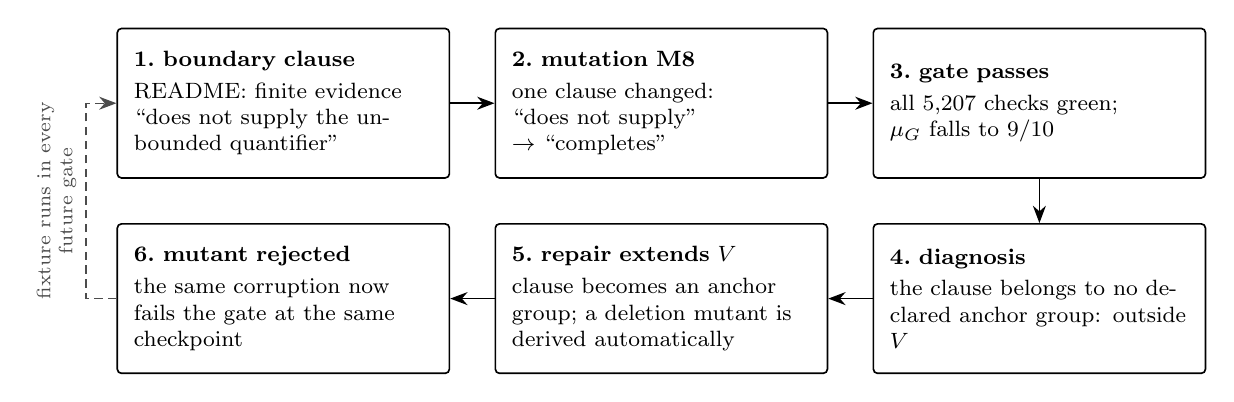
\begin{tikzpicture}[
  font=\footnotesize,
  stage/.style={draw, semithick, rounded corners=1.5pt, align=left,
    inner xsep=6pt, inner ysep=5pt, text width=10.8em, minimum height=5.4em},
  flow/.style={-{Stealth[length=2.2mm]}, semithick},
  back/.style={-{Stealth[length=2.2mm]}, densely dashed, gray!60!black}
]
\node[stage] (s1) {\textbf{1.\ boundary clause}\\[2pt]
  README: finite evidence ``does not supply the unbounded quantifier''};
\node[stage, right=1.6em of s1] (s2) {\textbf{2.\ mutation M8}\\[2pt]
  one clause changed:\\ ``does not supply''\\ $\to$ \mbox{``completes''}};
\node[stage, right=1.6em of s2] (s3) {\textbf{3.\ gate passes}\\[2pt]
  all $5{,}207$ checks green;\\ $\mu_G$ falls to $9/10$};
\node[stage, below=1.6em of s3] (s4) {\textbf{4.\ diagnosis}\\[2pt]
  the clause belongs to no declared anchor group: outside $V$};
\node[stage, left=1.6em of s4] (s5) {\textbf{5.\ repair extends $V$}\\[2pt]
  clause becomes an anchor group; a deletion mutant is derived automatically};
\node[stage, left=1.6em of s5] (s6) {\textbf{6.\ mutant rejected}\\[2pt]
  the same corruption now fails the gate at the same checkpoint};
\draw[flow] (s1) -- (s2);
\draw[flow] (s2) -- (s3);
\draw[flow] (s3) -- (s4);
\draw[flow] (s4) -- (s5);
\draw[flow] (s5) -- (s6);
\draw[back] (s6.west) -- ++(-1.1em,0) |- node[pos=0.25, rotate=90,
  font=\scriptsize, above, align=center] {fixture runs in every\\ future gate}
  (s1.west);
\end{tikzpicture}
\caption{The escape-to-fixture loop for mutation M8.  Stages 1--3 show the
enumeration boundary being crossed silently; stages 4--6 show the
architecture's repair idiom: the missing invariant is declared, the checker
derives its own rejection mutant from the declaration, and the corruption
becomes a permanent negative fixture.  The loop is the paper's contract
statement in miniature: declared boundaries are executable, undeclared
semantics are not.}
\label{fig:escape}
\end{figure}

\emph{What changed after the escape.}  The repair followed the architecture's
own idiom (Figure~\ref{fig:escape}).  The clause became a new anchor group in
the headline-status task of the comprehension checker, from which the suite
derives its deletion-rejection mutant automatically, so the escaped mutation
is now a permanent negative fixture.  At the same checkpoint, the repaired
checker passes the intact baseline and rejects the same corruption.  We did
not rerun the other nine mutations against the extended invariant family, so
no post-repair detection ratio is reported; the claim is only that this
corruption is now caught.

\emph{Threats to validity.}  The mutations were designed by the same author
as the checks, so this is a coverage demonstration, not an independent
red-team exercise.  One mutation per family says nothing about subtler
corruptions within a family: a status upgrade between adjacent rungs that
also regenerated the projections would pass the structural layer, as noted
above.  The study is $N=1$ in every sense that matters --- one corpus, one
maintainer, one working style.  There is no comparison against ordinary
continuous integration or against disciplined manual review, no measurement
of reader error with and without the architecture, no evidence that the
status taxonomy is complete, and no evidence that the byte budgets cause
comprehension rather than merely bounding bytes.

\subsection{Defects caught during development}\label{sec:receipts}

Three incidents from this corpus's own history, all public in the repository
record, show the same checks firing on real defects rather than planted ones.
They are ecological evidence and are reported separately from the controlled
study above.

First, boundary erosion: during a July 2026 editing pass, a wording
improvement to the README dropped the negative clause stating that an exact
final-skip band formula ``does not show that the actual orbit avoids'' an
unsafe band --- exactly the clause distinguishing a checked identity from the
open avoidance statement.  The cold-clone comprehension check failed the gate
within the same working session, and the sentence was restored before the
edit could land.

Second, attention overflow: the human orientation document reached $16{,}553$
bytes against a $16{,}000$-byte budget after new claim records landed, and
the bounded query summary reached $33{,}393$ bytes against $32{,}000$.  Both
overflows blocked the release gate and were resolved by removing duplicated
route text --- title-restating intent lines, per-route command strings
derivable from route identifiers --- rather than by raising either budget.

Third, coordinate rot at small scale: a five-line metadata addition to a
paper preamble shifted every subsequent line coordinate in that file; the
coordinate refresh and digest chain surfaced the stale projections
immediately, so the regenerated surfaces land with the edit rather than
after it.  Each incident is small; that is the point.  None of the three
would have announced itself, and two of the three were introduced by
tooling-assisted edits whose diffs looked entirely plausible in review.

\subsection{Cost}\label{sec:cost}

The complete machinery is $21$ Python files totalling $7{,}779$ lines, using
only the standard library, with no network access and no service
dependencies; the registry, methodology contract, and generated surfaces are
plain JSON and Markdown in the repository.  The full gate runs in about two
and a half minutes on commodity hardware ($144.5$ seconds at the evaluation
checkpoint), fast enough to run before every landing.
Maintaining the contract costs one structured edit per claim --- a status, a
declaration coordinate, a family assignment, and any open-obligation link.
We kept no time accounting, so no claim is made about maintenance cost
beyond the gate runtime and the implementation size just stated.

\section{What this architecture does not establish}\label{sec:limits}

This is a case study of one corpus, one maintainer, and one working style; no
controlled comparison against conventional practice was attempted, and a
disciplined author with ordinary continuous integration might avoid many of
the same defects at this scale.  The narrower claim defended here is that the
publication-faithfulness invariants of Sections~\ref{sec:authority}%
--\ref{sec:gate} are checkable at all, at commodity cost, and that they fired
on planted and on real defects.

The gate checks declared invariants, not meaning.  Anchored sentences are
protected; unanchored prose can still be mathematically inadequate in ways no
structural check will notice, which is why the methodology contract refuses
to let any semantic change class bypass human mathematical review, and why
the M8 escape is reported as the study's central result rather than as a
footnote.  The status taxonomy, anchor sentences, budgets, and family
partition are hand-designed for this corpus; nothing here automates the
judgement of which sentences are load-bearing, and no claim is made that the
taxonomy is complete or totally ordered.  Detection is not prevention: a
maintainer can still weaken a check, and the in-gate fixtures raise the cost
of doing so accidentally without making it impossible.  Finally, the proof
authority is inherited entirely from Lean and Mathlib; nothing in this paper
strengthens it, and kernel acceptance itself does not certify that a formal
statement captures its intended informal meaning --- that residue of
interpretation is exactly why the claim registry exists as a human-reviewed
object rather than a generated one.

\section{Related work}\label{sec:related}

\emph{Construction coverage and synchronisation.}  The closest Lean-native
relatives are formalisation blueprints.  Massot's
\texttt{leanblueprint}~\cite{leanblueprint} maintains a human-readable
account of a proof linked to its Lean formalisation, with a dependency graph
and per-node status; it has organised flagship developments including the PFR
formalisation~\cite{taopfr} and the Carleson project~\cite{carleson}.
LeanArchitect~\cite{leanarchitect} inverts the authoring direction,
extracting blueprint structure directly from annotated Lean and synchronising
the \LaTeX{} automatically.  Blueprints and this architecture answer
different questions at different times: a blueprint tracks \emph{coverage}
during construction --- which nodes of an intended proof are formalised ---
while the machinery here governs \emph{claim strength} at publication, a
concern that remains after coverage tracking ends and that applies to corpora
whose primary outputs include exact reductions and open boundaries rather
than a single target theorem.  The two compose naturally, and nothing here
replaces a blueprint.

\emph{Upstream semantic review.}  Lean Atlas~\cite{leanatlas} addresses the
complementary problem upstream of this one: whether formal statements
faithfully capture their intended mathematics, with dependency visualisation
that narrows the human review scope for AI-assisted formalisation.
Trustworthy Formal Natural Language Specifications~\cite{tfnls} goes further
for a controlled subset of English, producing proof certificates that explain
how each word of a specification was interpreted inside Lean.  Both establish
a stronger semantic connection than anything in this paper; both cover a
narrower prose form.  The present architecture checks ordinary human-authored
exposition structurally --- presence, anchoring, status agreement --- which
is semantically weaker and editorially broader.

\emph{Formal--informal document frameworks.}  Isabelle/DOF~\cite{isadof} is
the closest mature architectural antecedent: it defines document ontologies
over Isabelle documents that mix formal development and prose, and enforces
conformance continuously inside the IDE during document development and
evolution.  The differences are of object and time rather than ambition.
Isabelle/DOF governs a document's internal ontological structure as it is
edited; the machinery here governs a repository's \emph{external} publication
suite at release time --- a claim registry typed by logical strength with
explicit open obligations and non-claims, ordinary \TeX{} papers, and
generated projections that are not documents in the assistant at all --- and
its detectors are themselves mutation-tested.  Neither subsumes the other.

\emph{Library and archive maintenance.}  The Mathlib community
paper~\cite{mathlib} and \emph{Growing Mathlib}~\cite{growingmathlib}
describe the architecture and maintenance of a large general-purpose library
--- deprecation machinery, linters, review tooling, technical debt.  The
Archive of Formal Proofs~\cite{afp} demonstrates long-lived refereed
distribution of formal developments with sustained build guarantees.  Both
concern the health and acceptance of the formal artifact itself; the present
work takes that health as given and governs the faithfulness of what is
published \emph{about} it.

\emph{Documentation--code consistency.}  CASCADE~\cite{cascade} detects
inconsistencies between natural-language documentation and code by generating
unit tests from the documentation and executing them, flagging a mismatch
only when the real code fails a test that documentation-derived code passes.
Its evidence is behavioural and statistical where ours is deterministic and
provenance-rooted: the invariants here compare surfaces against a pinned
proof-assistant checkpoint rather than executing generated tests.

\emph{Evidence-gated research pipelines.}  Two recent systems gate research
claims on evidence and bind them into manuscripts.
ResearchLoop~\cite{researchloop} maintains a repository-backed claim ledger
with a claim-admission algorithm, so unaudited assertions cannot propagate
into the final paper, and evaluates on computational benchmarks.
XScientist~\cite{xscientist} treats a long-running autonomous research run as
a portable artifact carrying claim-to-evidence anchors, truth contracts,
content hashes, deterministic integrity forensics, and quality gates that can
block submission-ready status.  These are the nearest current systems in
spirit, and they rule out any claim that evidence-gated claim ledgers or
manuscript binding are new here.  The differences are the evidence root and
the vocabulary: in this corpus the root of trust is a pinned proof-assistant
checkpoint rather than recorded experiment executions, and the registry's
statuses encode the logical strength of mathematical statements ---
equivalence against implication, finite instance against unbounded claim,
open against cited --- together with explicit non-claims, for a
human-authored mathematics suite rather than an agent-generated research
artifact.

\emph{Mutation testing.}  Evaluating detectors by planting faults is a
standard method with a fifty-year history~\cite{demillo,jiaharman}; the
mutant--killed--survived vocabulary of Section~\ref{sec:eval} is standard
usage.  Nothing methodological is claimed there.  What is specific to this
paper is the mutation operators --- status upgrades, boundary-clause
weakenings, anchor manglings, budget paddings --- and the integration of
derived rejection mutants into the release gate itself.

\emph{The remaining conjunction.}  A July 2026 literature pass across
proof-assistant publication tooling, formal-document frameworks,
documentation-consistency checking, and AI-research control planes found the
ingredients of this architecture separately: claim ledgers with evidence
gates and paper bindings, continuously checked formal--informal documents,
certified prose-to-formal links, documentation-consistency testing, and
mutation-tested detectors.  We did not find a system combining a pinned
proof-assistant checkpoint, a typed registry of theorem status with explicit
open obligations and non-claims, ordinary authored mathematical prose
carrying verified source anchors, budgeted generated projections, and one
self-testing release gate over their agreement.  We make no stronger novelty
claim than that bounded, dated search, and we would be glad to learn of an
antecedent.

\section{Reusing the pattern}\label{sec:reuse}

Stated as commitments rather than code, the pattern evaluated here reads:

\begin{enumerate}
\item Record the authority order as data, and require every evidence class
  and every layer to state what it does not decide.
\item Make claim status a typed object: a closed taxonomy with structural
  rules, first-class open obligations with a closed effect vocabulary, and
  explicit non-claims --- including provenance non-claims if the public
  artifact projects a larger private effort.
\item Let authored prose carry verifiable coordinates inside readable words;
  pin links to immutable revisions; forbid floating references; and require
  every open obligation to own exactly one authored statement.
\item Generate every navigation surface from the registry, chain the layers
  with content digests, and put first-contact surfaces under byte budgets
  enforced at release.
\item Gate releases on all of the above with one cheap command, and give
  every checker negative fixtures that run inside the gate --- derived from
  the declared invariants where possible --- so the detectors are themselves
  under test.
\end{enumerate}

What does not transfer for free: the taxonomy, the anchor sentences, the
budgets, and the family partition are editorial judgements that must be
re-authored per corpus, and the implementation here is project-local script
rather than a reusable package.  Porting the pattern means re-authoring those
judgements and re-implementing the checks against a different corpus; we have
not measured that cost.  Whether the pattern transfers at all is untested ---
the commitments above are the portable statement of a design hypothesis whose
supporting evidence is one corpus.

\section{Complements and further questions}\label{sec:sys-further}

Four questions remain open on the engineering side.  Whether any useful
fraction of \emph{unanchored} prose adequacy can be checked --- beyond
presence of named sentences --- without drifting into checking style rather
than truth.  Whether the registry and contract vocabularies can be shared
across corpora without flattening exactly the distinctions that make a
per-corpus taxonomy honest.  Whether parts of the gate belong inside the
proof assistant itself, in the direction Isabelle/DOF takes for documents and
LeanArchitect for blueprints, rather than beside it in repository tooling.
And how the balance shifts as more of the editing pressure comes from AI
assistance: the incidents of Section~\ref{sec:receipts} suggest that as prose
generation gets cheaper, release-time faithfulness checking stops being
optional hygiene and becomes the load-bearing control, but one project's
history is evidence only that the failure mode is real, not that this is the
right general control.  The underlying mathematical corpus, meanwhile, keeps
its own open boundary: Erd\H{o}s problems 249 and 257 remain open, and every
surface this paper described exists to keep saying so exactly.

\begin{thebibliography}{99}
\bibitem{mainpaper} W.~Cook, \emph{Tail Certificates and Achievement-Set
Geometry for Erd\H{o}s Problems 249 and 257}, gateway exposition in this
release.
\bibitem{companion} W.~Cook, \emph{Finite-Difference Certificates and a
Phase-Separation Characterisation for Erd\H{o}s Problem 249}, companion note
in this release.
\bibitem{lean} L.~de Moura, S.~Kong, J.~Avigad, F.~van Doorn, and J.~von
Raumer, \emph{The Lean theorem prover}, in \emph{Automated Deduction ---
CADE-25}, Lecture Notes in Computer Science 9195, Springer, 2015,
pp.~378--388.
\bibitem{mathlib} The mathlib Community, \emph{The Lean mathematical
library}, in \emph{Proceedings of the 9th ACM SIGPLAN International
Conference on Certified Programs and Proofs (CPP 2020)}, ACM, 2020,
pp.~367--381, doi:\href{https://doi.org/10.1145/3372885.3373824}{10.1145/3372885.3373824}.
\bibitem{growingmathlib} A.~Baanen et al., \emph{Growing Mathlib:
maintenance of a large scale mathematical library}, in \emph{Intelligent
Computer Mathematics (CICM 2025)}, Lecture Notes in Computer Science,
Springer, 2026, \href{https://arxiv.org/abs/2508.21593}{arXiv:2508.21593}.
\bibitem{leanblueprint} P.~Massot, \emph{leanblueprint: a plasTeX plugin for
formalization blueprints},
\href{https://github.com/PatrickMassot/leanblueprint}{\texttt{github.com/PatrickMassot/leanblueprint}},
accessed July 2026.
\bibitem{leanarchitect} T.~Zhu, P.~Monticone, J.~Avigad, and S.~Welleck,
\emph{LeanArchitect: Automating Blueprint Generation for Humans and AI},
2026, \href{https://arxiv.org/abs/2601.22554}{arXiv:2601.22554}.
\bibitem{taopfr} T.~Tao, \emph{Formalizing the proof of PFR in Lean4 using
Blueprint: a short tour}, blog post, November 2023,
\href{https://terrytao.wordpress.com/2023/11/18/formalizing-the-proof-of-pfr-in-lean4-using-blueprint-a-short-tour/}{terrytao.wordpress.com}.
\bibitem{carleson} L.~Becker et al., \emph{A blueprint for the formalization
of Carleson's theorem on convergence of Fourier series}, 2024,
\href{https://arxiv.org/abs/2405.06423}{arXiv:2405.06423}.
\bibitem{afp} \emph{The Archive of Formal Proofs},
\href{https://www.isa-afp.org}{\texttt{isa-afp.org}}, accessed July 2026.
\bibitem{leanatlas} B.~Yanahama and A.~Sannai, \emph{Lean Atlas: An
Integrated Proof Environment for Scalable Human-AI Collaborative
Formalization}, 2026,
\href{https://arxiv.org/abs/2604.16347}{arXiv:2604.16347}.
\bibitem{tfnls} C.~S.~Gordon and S.~Matskevich, \emph{Trustworthy Formal
Natural Language Specifications}, in \emph{Proceedings of the 2023 ACM
SIGPLAN International Symposium on New Ideas, New Paradigms, and Reflections
on Programming and Software (Onward!\ 2023)}, ACM, 2023,
\href{https://arxiv.org/abs/2310.03885}{arXiv:2310.03885}.
\bibitem{isadof} A.~D.~Brucker and B.~Wolff, \emph{Isabelle/DOF: Design and
Implementation}, in \emph{Software Engineering and Formal Methods (SEFM
2019)}, Lecture Notes in Computer Science 11724, Springer, 2019,
pp.~275--292,
doi:\href{https://doi.org/10.1007/978-3-030-30446-1_15}{10.1007/978-3-030-30446-1\_15}.
\bibitem{cascade} T.~Kiecker, J.~A.~Sparka, M.~Reuter, A.~Ziegler, and
L.~Grunske, \emph{CASCADE: Detecting Inconsistencies between Code and
Documentation with Automatic Test Generation}, 2026,
\href{https://arxiv.org/abs/2604.19400}{arXiv:2604.19400}.
\bibitem{researchloop} Y.~Xia and T.~Wang, \emph{ResearchLoop: An
Evidence-Gated Control Plane for AI-Assisted Research}, 2026,
\href{https://arxiv.org/abs/2605.28282}{arXiv:2605.28282}.
\bibitem{xscientist} J.~Luo, \emph{XScientist: A Git-Like Research Protocol
for Long-Running Autonomous Scientific Discovery}, 2026,
\href{https://arxiv.org/abs/2607.12301}{arXiv:2607.12301}.
\bibitem{demillo} R.~A.~DeMillo, R.~J.~Lipton, and F.~G.~Sayward, \emph{Hints
on test data selection: Help for the practicing programmer}, IEEE Computer
11(4), 1978, pp.~34--41.
\bibitem{jiaharman} Y.~Jia and M.~Harman, \emph{An analysis and survey of the
development of mutation testing}, IEEE Transactions on Software Engineering
37(5), 2011, pp.~649--678.
\end{thebibliography}
\end{document}
